\chapter{Introduction}
\label{cha:intro}
The online social network (OSN) is the most impactful internet trend at the dawn of the 21st century. Words like tweeting, sharing, liking, trending and tagging have found common acceptance in the vocabulary of current internet users, while services like Facebook, Google+, LinkedIn and Twitter have become part of everyday life. OSNs offer millions of users an efficient and reliable channel to distribute and share information. At the same time, OSNs store large amounts of data which prompts several privacy concerns. In particular, it is possible to infer a considerable amount of sensitive information from the shared and stored content. Currently, users are allowed to configure ''privacy preferences'' in order to limit and select which users or groups can access the shared content. These preferences are generally too coarse-grained and difficult to configure~\cite{art:BonneauPS10}. Another problem is that these preferences do not exclude the provider along with the dangers of data leaks~\cite{art:Fischetti11} nor external governments~\cite{prism}.


%In May 2013, 72\% of all internet users were active on a social network~\cite{site:Jones13}. Currently, Facebook has 1.23 Billion monthly active users which corresponds to 17\% of the global population~\cite{site:Bullas14,site:worldometers}. Furthermore, the average Facebook user spends 15 hours and 33 minutes online per month~\cite{site:StatisticBrain}. These numbers show that social networks no longer represent the latest craze of an internet bubble. Conversely, OSNs are deeply rooted in our daily habits.

\section{Problem Statement}
\label{sec:problem_statement}
All these worrisome issues motivate the need for effective techniques to properly protect user's privacy in OSNs. Several solutions have been proposed and advocated to use cryptographic mechanisms in order to address the privacy issues, either by an add-on atop existing OSNs~\cite{art:BadenBSBS09,art:BeatoKW11,art:GuhaSTF08,art:LuoXH09}, or by complete new privacy-friendly architectures~ \cite{art:CristofaroSTW11}, mainly decentralised~\cite{art:CutilloMO11,NYT2010.Diaspora}. In general, those solutions suffer from user adoption and key management issues as users are required to register and then share, certify and store public keys~\cite{art:BalseBADG14}. Completely new architectures represent a difficult step for users as the trade off of moving away from the commonly used social ecosystem compared with the risk of losing interactions is high. Arguably, current centralised OSNs are here to stay and will continue to be actively used by millions of people. In light of recent events, such as Edward Snowden's whistle-blowing on US surveillance programs~\cite{prism}, OSN providers have all interest to maintain their users and a privacy-friendly image. However, not all OSNs are probably willing to cooperate in a more private infrastructure since an important part of their revenues consists of targeted advertising.

% Filipe's argumenten:
%        * OSN behoudt liever zijn gebruikers dan ze te verliezen omdat ze zich niet veilig voelen
%        * een groot deel van de OSN haar inkomsten komt van advertising aan een hele groep mensen, blijft nog steeds mogelijk
%        <-> wat met targeted advertising en behavioural analysis?

\section{Existing Solutions}
\label{sec:existing_solutions}
Earlier research has proposed peer-to-peer OSNs such as Safebook~\cite{art:CutilloMO11} and Diaspora~\cite{NYT2010.Diaspora}, in which no centralised authority has control over the network. However, these solutions face slow user adoption since users prefer not to face the risk of less social interaction in exchange for increased privacy in a completely new OSN environment. Therefore, only solutions to existing centralised OSN infrastructures are considered in the remainder of this text.

\paragraph{flyByNight~\cite{art:LucasB09}} is a Facebook application that protects user data by storing it in encrypted form on Facebook. It relies on Facebook servers for its key management and is thus not secure against active attacks by Facebook itself.

\paragraph{NOYB (None Of Your Business)~\cite{art:GuhaSTF08}} replaces details of a user with details from other random users thereby making this process only reversible by friends. However, the proposed solution does not apply to user messages or status updates that are the most frequently used features in the OSNs considered in this thesis.

\paragraph{FaceCloak~\cite{art:LuoXH09}} stores published Facebook data on external servers in encrypted form and replaces the data on Facebook with random text from Wikipedia. This could be a useful mechanism to prevent OSNs from blocking security aware users because they are scared to see their advertising revenues shrink. However, this approach has the disadvantage that other users could take this data as genuine user content which may lead to social issues. Furthermore, FaceCloaks architecture leads to an inefficient key distribution system.

\paragraph{Persona~\cite{art:BadenBSBS09}} is a scheme that can be used as a Firefox extension to let users of an OSN determine their own privacy by supporting the ability to encrypt messages to a group of earlier defined friends based on \textit{attribute-based encryption} (ABE)~\cite{art:SahaiW04}. The scheme supports a wide range of meaningful use cases. For instance, sending messages to all friends that are related to a certain attribute or even encrypting messages to friends of friends. However, the major drawback of this system is that, for every new friend  a public key is exchanged before he is able to interact in the privacy preserving architecture consequently requiring an infrastructure for broadcasting and storing public keys. Furthermore, to support the encryption of messages to friends of friends, user defined groups should be made available publicly thereby making the public key distribution system even more complicated. Finally the proposed ABE encryption scheme is 100 to 1000 times slower than a standard RSA operation~\cite{art:BadenBSBS09}.

\paragraph{Scramble~\cite{art:BeatoKW11}} is a Firefox extension that allows users to define groups of friends that are given access to stored content on OSNs. The tool uses public key encryption based on OpenPGP~\cite{rfc4880} to broadcast encrypted messages on any platform. Furthermore Scramble provides the implementation of a tiny link server such that OSN policies not allowing to post encrypted data are bypassed. However, as indicated by usability studies~\cite{art:WhittenT99} OpenPGP has a higher usage threshold because an average user does not manage to understand OpenPGP properly. Additionally, Scramble has to rely on the security decisions of the web of thrust. It therefore inherits the unpleasant property of OpenPGP that the user can not be sure that the used PGP key actually belongs to the intended Facebook profile.

However, the most unattractive property of all centralised applications is that they have to rely on a rather complex infrastructure. Persona has to support an extended public key distribution system and Scramble relies on the leap-of-faith OpenPGP web of trust. All proposed solutions require users with no cryptographic background on asymmetric cryptography to make responsible decisions concerning the management of their keys. Furthermore, maintaining such complex key infrastructures becomes more and more complex as more users subscribe.

\section{Goals}
\label{sec:goals_of_this_thesis}
The goal of this thesis is to develop an architecture that solves the aforementioned issues thereby taking the challenges and pitfalls from earlier solutions into account. Specifically, the architecture should present the following properties:
\begin{itemize}
 \item \textbf{User friendly:} The average OSN user should be able to use the resulting architecture, i.e. a user with no knowledge on cryptographic primitives.
 \item \textbf{Applicable:} The original OSN environment should not be altered since some OSN providers are probably not willing to support a more confidential architecture because it could possibly hurt their business model.
 \item \textbf{Immediately ready to use:} No additional registration or subscription to third party key architectures should be required to enable usage of the system. As soon as a user subscribes to the OSN provider he should be able to start receiving confidential messages.
\end{itemize}

\section{Main Idea}
Identity Based Encryption (IBE)~\cite{art:Shamir84} solutions overcome the key management problem as the public key of the user can be represented by any valid string, such as the email, unique \id{} and username. Therefore, by using an OSN username any savvy and concerned user can share encrypted content with other users who are not using the solution, thereby motivating curious ones to use the system as well. Nevertheless, IBE-based systems require a trusted central Private Key Generator (PKG) server to generate the private parameters for each user based on a master secret. Consequently, such an architecture only shifts the trusted party from the OSN to the PKG. However, this problem can be mitigated if the master secret is divided among multiple PKGs following a Distributed Key Generation (DKG)~\cite{art:Pedersen91a} protocol based on Verifiable Secret Sharing (VSS)~\cite{art:ChorGMA85}. A DKG protocol allows $n$ entities to jointly generate a secret requiring that a threshold $t$ of the $n$ entities does not get compromised. In fact, each entity holds only a share of the master secret, that can be reconstructed by at least $t$ shares. 

Many OSN users are not only represented on a single OSN but on several, thus, can also hold multiple public keys. Moreover, the multi-PKG setting could be supported and maintained by different organisations, each with their own motivations to support more private OSNs. In particular, if OSN providers see their advertisement revenues drop due to privacy concerned users deleting their profiles, they have an incentive to support and maintain such a multi-PKG setting. Since collaboration between OSN providers that compete along is assumed to be a difficult task and orthogonal to their economical business model, the different PKGs do not compromise the security of the DKG protocol. Figure~\ref{fig:overview} depicts an overview example of a possible model, where a user authenticates to $t$-PKGs of his choice using, e.g. a similar token as in open id protocols, to retrieve his private key. This action can be performed after the reception of encrypted content as a consequence of user curiosity. The PKG servers can also be represented by governmental entities or subsidised research institutions from different continents, with no incentives to collaborate nor overcome more powerful adversaries using legal measures~\cite{art:Matyszcyk12} among at least $t$-PKGs. 

\begin{figure}[ht]
    \begin{center}
    \scalebox{0.78}{
        \begin{tikzpicture}[auto, node distance=1mm,
            block/.style={rectangle,text width=6em,text centered,minimum height=11mm},
            line/.style={draw,very thick, ->},
            line2/.style={draw,very thick, <->},
            leg/.style={font=\scriptsize,text centered},
            ]
            % \draw[help lines] (-6,-5) grid (8,3);
            \draw[dashed] (-5,6) -- (5,6) -- (5,3) -- (-5,3) -- (-5,6);
            \path
                % title of PKG BOX
                (0, 6.5) node {\textbf{Pool of Multiple PKGs}}
                
                % Bottom part
                (-5.5,0) node [block] (user) {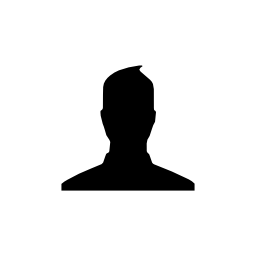
\includegraphics[scale=0.2]{img/fbuser.png}}
                (0,0) node [block] (fb) {
\includegraphics[scale=0.12]{img/fb_icon.png}}
                (5.5, 0) node [block] (friends) {
\includegraphics[scale=0.3]{img/fbfriends.png}}

                %Top part (PKG lists)
                (-3,4) node [block] (linkedin) {
\includegraphics[scale=0.1]{img/linkedin.png}}
                (-4,5) node [block] (fbpkg) {
\includegraphics[scale=0.06]{img/fb_icon.png}}
                (1.2,5) node [block] (gplus) {
\includegraphics[scale=0.08]{img/gplus.png}}
                (-2,5.2) node [block] (tumblr) {
\includegraphics[scale=0.1]{img/tumblr.png}}
                (2.8,4) node [block] (pin) {
\includegraphics[scale=0.05]{img/pinterest.png}}
                (4.2,5) node [block] (tor) {
\includegraphics[scale=0.1]{img/tor.png}}
                (-0.5,4) node [block] (twitter) {
\includegraphics[scale=0.05]{img/twitter.png}};

            \node[below=of fb] {\textbf{Facebook}};
            \node[below=of user] {\textbf{User}};
            \node[below=of friends] (frdcaption) {\textbf{Subset of Recipients}};
            \node[below=of frdcaption] {\textbf{s.t., $\mathcal{S}=\{\id{1},\id{2},\ldots,\id{\eta}\}$}};


            \begin{scope}[every path/.style=line]
                \path (user.east) -- (fb.west);               
            \end{scope}   

            % Legend
            \path (-2.8,0.35) node [leg] {Publish: $C\leftarrow$ Encrypt($m$,$\mathcal{S}$)};
            \path (2.7,0.35) node [leg] {Retrieve $C$};
            \node[right=of friends] {Decrypt($C$)};
                
            \begin{scope}[every path/.style=line2]
                \path (fb) -- (friends);
                \path[dashed] (friends.north) -- (tor.south);
                \path[dashed] (5.1,1) -- (3.1,3.4);
                \path[dashed] (4.7,0.95) -- (0.5,3.5);
            \end{scope}
        \end{tikzpicture}
    }
    \end{center}
    \caption{Multiple $(n,t)$-PKG IBE for OSNs overview, for a message $m$ published for the set $\mathcal{S}$ for $t=3$. The PKG infrastructure can be maintained by virtually any organisation with an incentive to make OSNs more private.}
    \label{fig:overview}
\end{figure}

\section{Structure of this Thesis}

The structure of this thesis is organised as follows:
%Chapter~1 situates the prominent role Online Social Networks (OSNs) take in our daily life and labeled the currently offered privacy preferences as insufficient for the protection of users' data. Existing solutions providing an answer to these issues were briefly discussed along with their drawbacks and why none of these solutions has found common acceptance in the online community of OSNs. This allowed the definition of general design goals a practically usable architecture should achieve in order to increase user acceptance. These objectives of user friendliness, applicability and immediate usability are the guidelines for the design of an improved architecture.
\begin{description}
 \item[Chapter~2] introduces required mathematical background such as definitions on complexity theory, algebraic groups, finite fields and number theoretic assumptions. From the Computational Diffie-Hellman problem (CDH) and the Decisional Diffie-Hellman problem (DDH), the Gap Diffie-Hellman problem (GDH) follows naturally. Bilinear maps are introduced as a response to GDH in the form of a practically usable DDH oracle. The notion of bilinear maps then allows to derive the Bilinear Diffie-Hellman problem (BDH) which guarantees the security of our future constructions. The chapter concludes with basic definitions and notations on cryptography along with hash functions and the random oracle assumption.

 \item[Chapter~3] highlights all cryptographic building blocks for the design of our solution. The chapter starts with a review on traditional public key infrastructures (PKI). An elaborate discussion on identity-based encryption (IBE) follows, describing a comparison of IBE and PKI, security notions of IBE, a summary of literature on IBE and the most attractive IBE schemes proposed in literature. Consequently, the reader is introduced to broadcast encryption and secret sharing. Chapter~3 concludes with distributed key generation as an anonymous generalisation of secret sharing.

 \item[Chapter~4] describes the design of a practical encryption scheme for OSNs. We start by defining a model which describes the current OSN situation. With the help of this model, the current security threats are uncovered along with possible adversaries and realistic assumptions on these adversaries. Chapter~4 continues by defining different cryptographic design goals to resolve the earlier described security threats. The design goals serve as a guideline to construct a practical algorithm with the help of the cryptographic building blocks from Chapter~3. The end of Chapter~4 proposes a mathematical Algorithm that is the result of our earlier design decisions.

 \item[Chapter~5] discusses the practical details of implementing the algorithm derived in Chapter~4 as a proof-of-concept. First, an introduction is given on Scramble, an existing tool for broadcast encryption in OSNs. This is followed by adaptations to the existing architecture in order to implement our algorithm from Chapter~4. Chapter~5 further discusses the practical implementation decisions along with the structure of our code. This is followed by a performance analysis of the implementation. The last section of Chapter~5 presents the current limitations of our proof-of-concept.

 \item[Chapter~6] concludes this thesis with a summary of earlier research results along with the limitations of our current solution. Finally, we conclude this thesis by highlighting topics that might be subject of future work along with the wide plethora of applications our construction might enable.

\end{description}

%%% Local Variables: 
%%% mode: latex
%%% TeX-master: "thesis"
%%% End: 
